\chapter{Databases and Database Users}

\subsection{Introduction}

A \textbf{database} is a collection of related data. By
\textbf{data}, we mean known facts that can be recorded and
have implicit meaning. This is a very general defination.\\

A database has the following implicit properties:

\begin{itemize}
    \item Database represent some aspect of the real world,
        call its \textbf{Universe of Discourse (UoD)}.
    \item Database is a lofically coherent collection of data
        with some inherent meaning.
    \item It has a specific purpose.
\end{itemize}

A \textbf{database management system (DBMS)} is a computerized
system the enables users to create and maintain a database. The 
DBMS facilitates the following jobs:

\begin{itemize}
    \item \textbf{Defining} a database involves specifying the
        data types, structures and constraints of the data
        to be stored in the database. The database definition 
        or descriptive information is also
        stored by the DBMS in the form of a database
        catalog or dictionary; it is called
        textbf{meta-data}.
    \item \textbf{Constructing} the database is the process of
        storing the data on some storage medium controlled by the
        DBMS.
    \item \textbf{Manupulating} a database includes
        quering, updating, generating reports.
    \item \textbf{Sharing} a database allows multiple users
        to access it simultaneously.
\end{itemize}

An \textbf{application program} accesses the database by sending
queries or requests for data to DBMS.\\

A \textbf{query} typically causes some data to be retrieved.\\

\textbf{Protection} includes \textit{system protection} against
hardware or software malfunction and \textit{security protection}
against unauthorized or malicious access.\\

The DMBS must be able to \textbf{maintain} the database system by
allowing the system to evolve as requirements change over time.\\

Together a database and DBMS software form a \textbf{database
system}.

\begin{figure}[h!]
    \begin{center}
        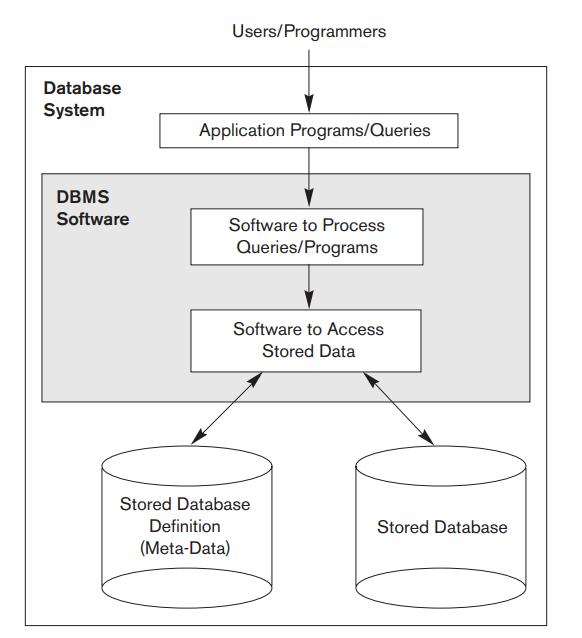
\includegraphics[width=7cm]{fig1.png}
        \caption{A simplified database system environment}
    \end{center}
\end{figure}

\subsection{Characteristics of the Database Approach}

\begin{itemize}
    \item \textbf{Self-Describing Nature of a Database System}\\
        A database system contains a complete defination of
        the database structure and contraints. This defination
        is stored in the DBMS catalog. The information stored
        in the catalog is called \textbf{meta-data}, and it
        describes the structure of primary database. Some systems
        such as NOSQL systems, do not require meta-data as they
        store \textbf{self-describing data} that includes the
        data info and data in one structure.

    \item
\end{itemize}
